\PID
У поједностављеном дигиталном комуникационом систему се информације преносе као сигнали дискретни у времену. 
Услед ефеката преноса информација обично се дешава да информација која се 
преноси у једном тренутку, задржавајући се на неки начин у каналу\footnote{Што значи да је такав канал систем са меморијом, у случају 
електричног канала узрок су на пример реактивни елементи, а у случају преноса у оптичком влакну узрок је дисперзија.}, утиче на излаз и у неколико наредних 
тренутака. Да би се то кориговало, користи се \textit{еквилајзер} - филтар за обликовање сигнала тако да се поништи овај ефекат. Познато је да је импулсни
одзив канала $h[n] = \updelta[n] + 0,4 \updelta[n-1]$. Односно, један импулс на улазу производи импулс на излазу као и још један мањи импулс, један 
тренутак касније. 
\begin{enumerate}[label=(\alph*)]
\item Одредити преносну функцију филтра $F(z)$ који треба поставити након канала, тако да се поништи описани ефекат, односно, да се информације на 
излазу не преклапају. 
\item Одредити импулсни одзив тог филтра у временском домену и графички приказати добијени резултат. 
\item Реализовати такав филтар помоћу идеалних блокова за кашњење и множача. 
\end{enumerate}

\RESENJE
(а) Функција преноса канала одређује се као $\mathcal{Z}$-трансформација импулсног одзива\footnote{
    Користи се таблична трансформација \ref{T:ZT:delta}, као и правило о померању у времену. 
} према 
\begin{eqnarray}
    H(z) = \ZT{h[n]} = \ZT{\updelta[n]} + 0,4 \ZT{\updelta[n-1]} 
                     = 1 + 0,4\dfrac{1}{z} = \dfrac{0,4 + z}{z}.
\end{eqnarray}
Каскадна веза датог канала и еквилајзера је функција преноса која је производ појединачних функција преноса као 
\begin{eqnarray}
    W(z) = H(z) F(z)
\end{eqnarray}
Оно што је познато, јесте да еквилајзер треба да поништи ефекте канала, односно треба да буде као да сметњи које је додао канал није ни било, 
односно $W(z) = 1$, тиме је\footnote{Ова техника се назива и инверзно филтрирање, видети и задатак \refz{pz_cancel}}
\begin{eqnarray}
    F(z) = \dfrac{1}{H(z)} = \dfrac{z}{0,4 + z}
\end{eqnarray}

(б) Користећи таблични резултат \ref{T:z:exp} добија се импулсни одзив филтра у временском домену
\begin{eqnarray}
    f[z] = \IZT{F(z)} = \IZT{\dfrac{z}{z-\underbrace{(-0,4)}_a} } = (-0,4)^n \uu[n]
\end{eqnarray}
Добијени резултат приказан је на слици \ref{fig:\ID.1}
%

\begin{figure}[t!]
    \centering
        \begin{subfigure}{0.59\textwidth}
            \centering
            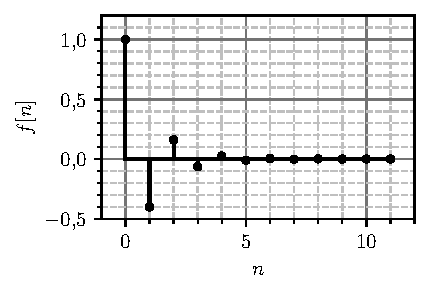
\includegraphics{fig/h_equalizer.pdf}
            \caption{Импулсни одзив филтра $f[n]$.}
            \label{fig:\ID.1}
        \end{subfigure}
        %
        \begin{subfigure}{0.39\textwidth}
            \centering
            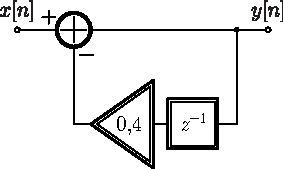
\includegraphics{fig/equalizer_blok.pdf}
            \caption{Реализација задатим компонентама.}
            \label{fig:\ID.2}
        \end{subfigure}
        \caption{Уз решење задатка.}
    \end{figure}
%
(в) Функцију преноса треба изразити у облику који је погодан за реализацију. Будући да је функција преноса блока за кашњење
$z^{-1}$ треба изразити све чланове у том облику.
Сама функција преноса филтра представља однос одзива и побуде па је $F(z) = \dfrac{Y(z)}{X(z)} = \dfrac{z}{0,4 + z} = 
\dfrac{1}{1 + 0,4 z^{-1}}$. Даље је $Y(z) (1 + 0,4 z^{-1}) = X(z)$, па се одзив може изразити као 
\begin{equation}
    Y(z) = X(z) - 0,4 z^{-1} Y(z)
\end{equation}
На основу тога, дати филтар се може реализовати како је приказано на слици \ref{fig:\ID.2}.
